\documentclass[a4paper,landscape]{article}
% dummy change
\usepackage{geometry}
\usepackage{tikz}
\begin{document}
\thispagestyle{empty}
\centerline{\bfseries Dependency Tree of \TeX\ live packages for Debian}

\bigskip
\[
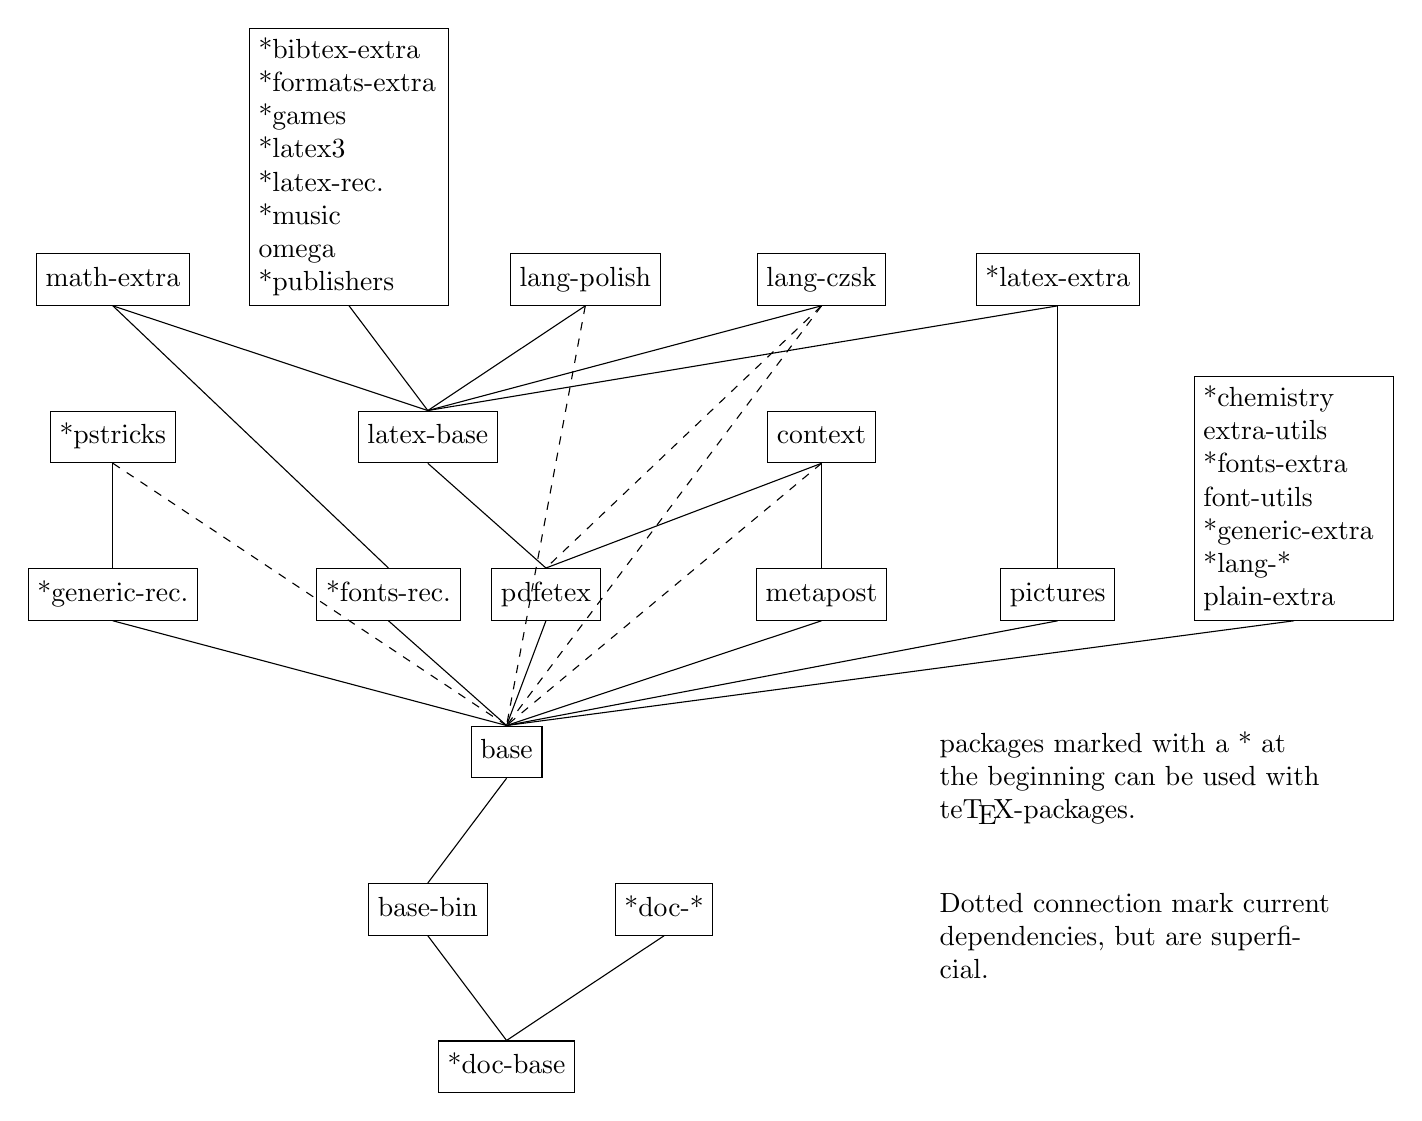
\begin{tikzpicture}
  \node[above] (doc-base)	at (5,-2)	[draw]	{{*}doc-base\strut};
  \node[above] (base-bin)	at (4,0)	[draw]	{base-bin\strut};
  \node[above] (doc)		at (7,0)	[draw]	{{*}doc-{*}\strut};

  \node[above] (base)		at (5,2)	[draw]	{base\strut};
  
  \node[above] (generic-rec)	at (0,4)	[draw]	{{*}generic-rec.\strut};
  \node[above] (fonts-rec)	at (3.5,4)	[draw]	{{*}fonts-rec.\strut};
  \node[above] (pdfetex)	at (5.5,4)	[draw]	{pdfetex\strut};
  \node[above] (metapost)	at (9,4)	[draw]	{metapost\strut};
  \node[above] (pictures)	at (12,4)	[draw]	{pictures\strut};
  \node[above] (generic-extra)	at (15,4)	[draw]	{%
  	\parbox[t]{2.3cm}{%
		       {*}chemistry\\
		       extra-utils\\
		       {*}fonts-extra\\
		       font-utils\\
			{*}generic-extra\\
		       {*}lang-*\\
		       plain-extra}};

  \node[above] (pstricks)	at (0,6)	[draw]	{{*}pstricks\strut};
  \node[above] (latex-base)	at (4,6)	[draw]	{latex-base\strut};
  \node[above] (context)	at (9,6)	[draw]	{context\strut};

  \node[above] (math-extra)	at (0,8)	[draw]	{math-extra\strut};
  \node[above]	(bibtex-extra)	at (3,8)	[draw]	{%
  	\parbox[t]{2.3cm}{{*}bibtex-extra\\
		       	{*}formats-extra\\
			{*}games\\
			{*}latex3\\
			{*}latex-rec.\\
			{*}music\\
		        omega\\
			{*}publishers}};
  \node[above] (lang-polish)	at (6,8)	[draw]	{lang-polish\strut};
  \node[above] (lang-czsk)	at (9,8)	[draw]	{lang-czsk\strut};
  \node[above] (latex-extra)	at (12,8)	[draw]	{{*}latex-extra\strut};

  \draw (base.south) -- (base-bin.north);
  \draw (base-bin.south) -- (doc-base.north);
  \draw (doc.south) -- (doc-base.north);

  \draw (generic-rec.south) -- (base.north);
  \draw (fonts-rec.south) -- (base.north);
  \draw (pdfetex.south) -- (base.north);
  \draw (metapost.south) -- (base.north);
  \draw (pictures.south) -- (base.north);
  \draw (generic-extra.south) -- (base.north);

  \draw (pstricks.south) -- (generic-rec.north);
  \draw (latex-base.south) -- (pdfetex.north);
  \draw (context.south) -- (pdfetex.north);
  \draw (context.south) -- (metapost.north);

  \draw (math-extra.south) -- (fonts-rec.north);
  \draw (math-extra.south) -- (latex-base.north);
  \draw (bibtex-extra.south) -- (latex-base.north);
  \draw (lang-polish.south) -- (latex-base.north);
  \draw (lang-czsk.south) -- (latex-base.north);
  \draw (latex-extra.south) -- (latex-base.north);
  \draw (latex-extra.south) -- (pictures.north);

  \draw[dashed] (pstricks.south) -- (base.north);
  \draw[dashed] (lang-polish.south) -- (base.north);
  \draw[dashed] (lang-czsk.south) -- (pdfetex.north);
  \draw[dashed] (lang-czsk.south) -- (base.north);
  \draw[dashed] (context.south) -- (base.north);

  \draw (13,2) node[text width=5cm] {packages marked with a * at the beginning can be used with te\TeX-packages.};
  \draw (13,0) node[text width=5cm] {Dotted connection mark current dependencies, but are superficial.};
\end{tikzpicture}
\]
\end{document}

